% Source: team draft v0.11. Compile twice with pdflatex or use latexmk -pdf paper.tex.
\documentclass[conference,a4paper]{IEEEtran}
\usepackage[T1]{fontenc}
\usepackage{amsmath,amssymb,graphicx,booktabs,url}
\usepackage{xcolor,soul}
% Remove the wrapper after revising a highlighted passage.
\newcommand{\pendingedit}[1]{\hl{#1}}
\usepackage[hidelinks]{hyperref}
\title{DUAL: Dual Ocular Screener for Cataract and Glaucoma Triage from Fundus Photographs}
\author{\IEEEauthorblockN{Anel Bazarbayeva, Negar Kamvij, Shridhi Patel, Bhoami Khona,\\
Krushiben Patel, Ansh Kevadiya, Smit Meghapara}
\IEEEauthorblockA{Seidenberg School of Computer Science and Information Systems\\
Pace University, New York, NY, USA\\
\texttt{ab21376n@pace.edu, nk13719n@pace.edu, sp17432n@pace.edu, bk10823n@pace.edu}\\
\texttt{kp85462n@pace.edu, ak61253n@pace.edu, sm76879n@pace.edu}}}
\begin{document}
\maketitle
\begin{abstract}

Cataract and glaucoma are leading causes of blindness, and both leave signs on a colour fundus
photograph, although cataract appears only indirectly, as reduced image clarity. We present DUAL, a
triage aid that screens a single photograph for both conditions using a ResNet-50 backbone shared by
two binary heads. For each condition it returns No concern, Refer, or Uncertain, refer. The models
were trained on eye-level labels derived from ODIR-5K. Calibration, decision thresholds with a 90\%
sensitivity floor and an abstention band were fitted on the internal validation split and frozen
before any testing. On the internal test split, the application model reached an AUROC of 0.995 for
cataract and 0.921 for glaucoma, and the shared backbone performed as well as separate
single-disease models, although neither design was consistently better on external data. On four
public external data sets scored with the frozen settings, performance dropped. The cataract AUROC
was 0.909 on retina\_dataset\_2016, and the glaucoma AUROC ranged from 0.760 to 0.869 on full fundus
photographs but was near chance on the tightly cropped ACRIMA set. Sensitivity fell below the
validation floor, and the calibrated probabilities were far too low. In the shortcut checks, the
cataract head referred most hazy or strongly blurred photographs without cataract, and the strongest
point of the glaucoma heatmap fell inside the optic disc in 37\% of ORIGA and 67\% of DRISHTI-GS
photographs. \pendingedit{DUAL is a research prototype, and these external results and shortcut checks show what
must improve before it could be used clinically. [Pending: update once the frozen model is connected
to the application.]}

\end{abstract}
\begin{IEEEkeywords}

cataract, glaucoma, fundus photography, deep learning, multi-task learning, external validation,
calibration, Grad-CAM, triage

\end{IEEEkeywords}

\section{Introduction}

In 2020, cataract and glaucoma were the two leading causes of blindness worldwide among adults aged
50 and older, with an estimated 15.2 million and 3.6 million blind people, respectively, and
cataract was also the second leading cause of moderate and severe vision impairment \cite{ref1}.
Early detection matters for both conditions, but for different reasons. Cataract is treatable, so
the vision loss it causes counts as avoidable \cite{ref1}, yet many visually significant cases go
undiagnosed where screening is hard to reach \cite{ref2}. Glaucoma is the leading cause of
irreversible blindness. About 64.3 million people aged 40 to 80 had glaucoma in 2013, a number
projected to reach 111.8 million by 2040 \cite{ref3}, and in population studies more than half of
glaucoma cases had not been detected before \cite{ref4}.

Colour fundus photographs are quick to acquire and are already collected in diabetic retinopathy
screening programmes \cite{ref5}. Deep learning systems trained on these photographs have detected
possible glaucoma \cite{ref5}, glaucomatous optic neuropathy \cite{ref6}, \cite{ref7} and visually
significant cataract \cite{ref2} with high AUROC. However, most of these systems address one disease
at a time, and many report their best results on data from the same source as their training data.
External validation of cataract models has been limited \cite{ref8}, and glaucoma models trained at
a single clinic often lose accuracy on other data sets \cite{ref9}.

In this paper we present DUAL, a triage aid that screens one fundus photograph for both cataract and
glaucoma. A ResNet-50 backbone is shared by two binary heads, and each head gives a separate result:
No concern, Refer, or Uncertain, refer. DUAL is intended to help decide who should be seen by an eye
specialist. It does not make a diagnosis.

The main contributions of this work are as follows: (1) eye-level labels and a patient-level split
of ODIR-5K, with borderline cases (suspected glaucoma, media opacity and poor image quality) held
out for targeted checks; (2) a multi-task versus single-task ablation over three seeds using the
same training loop; (3) calibration, decision thresholds and an abstention band fitted on internal
validation only and frozen before any test data were scored; (4) external validation on four public
data sets that were never used for training, scored with the frozen settings; (5) shortcut checks,
consisting of a haze check on media-opacity eyes, a synthetic blur test and Grad-CAM \cite{ref10}
heatmaps of the cataract and glaucoma outputs, including an optic disc check; and \pendingedit{(6) a prototype
web application for the screening workflow, which still uses a mock scoring model until the frozen
model is connected. [Pending: update once the frozen model is connected to the application.]}

Section II reviews related work. Sections III to V describe the data, labels and preprocessing,
Sections VI and VII cover the model, training and calibration, and Section VIII reports the results.
Section IX describes the application, Section X discusses the limitations, and Section XI concludes
with directions for future work.

\section{Literature Review}

Glaucoma detection from fundus photographs has been widely studied. Li et al. \cite{ref6} trained a
deep learning system on 48,116 photographs graded by 21 ophthalmologists and reported an AUROC of
0.986 for referable glaucomatous optic neuropathy on 8,000 validation photographs. About half of the
false negatives in their study had coexisting eye conditions, mostly high or pathologic myopia. Ting
et al. \cite{ref5} reported an AUROC of 0.942 for possible glaucoma in a national diabetic
retinopathy screening programme. Christopher et al. \cite{ref11} compared several architectures on
14,822 photographs and found that transfer learning from ImageNet improved accuracy and shortened
training, reaching an AUROC of 0.91. Diaz-Pinto et al. \cite{ref12} fine-tuned five ImageNet models,
including ResNet-50, tested them across the public glaucoma data sets available to them, and
released ACRIMA, which serves here as one of the external test sets.

Cataract has received less attention than diabetic retinopathy, age-related macular degeneration or
glaucoma, and Goh et al. \cite{ref8} noted in a review that cataract studies were often limited by a
lack of robust, high-quality training data and of external validation. Zhang et al. \cite{ref13}
applied a deep convolutional network to fundus photographs and reported accuracies of 93.52\% for
cataract detection and 86.69\% for grading. Tham et al. \cite{ref2} trained a model on more than
25,000 retinal photographs from population studies to detect visually significant cataract, with an
internal AUROC of 0.966 and AUROCs of 0.916 to 0.965 in three external studies. Because a fundus
photograph shows cataract only indirectly, through reduced clarity of the retinal image, a model may
also respond to haze from other causes. This possibility motivated the media-opacity and blur checks
in Section VIII-E.

Multi-task learning trains related tasks together on a shared representation, which can help each
task generalise \cite{ref14}. In ophthalmology, Cen et al. \cite{ref15} built a platform trained on
249,620 photographs that detects 39 fundus diseases and conditions, and ODIR-5K was released
together with a benchmark for recognising eight diagnostic categories from paired fundus photographs
\cite{ref16}. DUAL limits the problem to two conditions and compares the shared model directly with
single-disease models trained in the same way.

Models that perform well on their own data can do worse elsewhere. Zech et al. \cite{ref17} found
that a pneumonia model trained on chest radiographs from two hospital systems dropped from an AUROC
of 0.931 on internal data to 0.815 at a third hospital system. For glaucoma, Hemelings et al.
\cite{ref9} noted that single-clinic models often struggle on external data because glaucoma
prevalence, cameras and the definition of glaucoma differ. Their G-RISK model, which uses
standardised disc-centred images, kept high performance across 13 data sources, with AUROCs of 0.976
and 0.984 in two population cohorts. Liu et al. \cite{ref7} similarly tested a glaucoma system on
clinical, population-based and web-sourced photographs.

Accuracy alone does not show that a model relies on the right evidence. Models can learn shortcuts,
that is, decision rules that perform well on standard benchmarks but fail to transfer to more
demanding test conditions \cite{ref18}. DeGrave et al. \cite{ref19} showed that COVID-19 radiograph
models relied on such confounders and that external testing alone may not reveal them. Heatmap
methods such as Grad-CAM \cite{ref10} help to inspect which image regions a model attends to. Modern
neural networks are also often poorly calibrated \cite{ref20}, and Leibig et al. \cite{ref21} showed
for diabetic retinopathy that referring the most uncertain decisions for further review improved
performance on the remaining cases. The present study screens two conditions from one photograph and
combines a matched multi-task ablation, calibration and abstention fixed before testing, external
validation on four public data sets, and explicit shortcut checks.

\section{Data}

DUAL was trained only on the ODIR-5K data set \cite{ref16}, using its 3,500 labelled training
patients with one fundus photograph of each eye, or 7,000 photographs in total. Labels were assigned
per eye, as described in Section IV. To measure how well the models perform on photographs from
other sources, four further data sets were used for testing only and never for training, tuning or
calibration. ORIGA \cite{ref22} (650 images), DRISHTI-GS \cite{ref23} (101 images) and ACRIMA
\cite{ref12} (705 images) were used to test glaucoma detection. The retina\_dataset\_2016 data set
\cite{ref24} (601 images), a public collection with no documented clinical source, served as the
only external cataract test set and also provided 101 glaucoma images. We screened other public
fundus data sets but did not use them, mainly because they lack a cataract label, were built partly
from ODIR-5K, or require institutional access. An MD5 comparison found no exact duplicate images
between ODIR-5K and retina\_dataset\_2016. All data sets were used for non-commercial academic
research only.

\section{Labels and Splits}

ODIR-5K provides 3,500 patient records, each with a left-eye and a right-eye fundus photograph. We
generated 7,000 eye-level records from each eye's own diagnostic keyword field instead of the
patient-level disease columns, so that a condition recorded for only one eye is not assigned to
both. The resulting labels identify 313 cataract-positive eyes and 282 eyes with confirmed glaucoma.
Separate flags record suspected glaucoma, media opacity, image-quality concerns and unusable images.

Eyes that needed separate safety evaluation were placed in a common holdout split: 63 media-opacity
eyes for the cataract haze shortcut check, 44 suspected-glaucoma eyes because their disease status
is uncertain, and 21 low-image-quality eyes to evaluate the ``Uncertain, refer'' outcome. Four
media-opacity eyes were also suspected of glaucoma, so the holdout contains 124 unique eyes. Nine
further unusable images were excluded. Placing one eye in the holdout did not remove the fellow eye
from the training, validation and test splits. This kept the main splits at their planned size, but
it means that some holdout patients have their other eye in training. The haze check therefore
reports these patients separately (Section VIII-E), and a future split should hold out both eyes.

Eligible eyes were divided into training, validation and internal test sets at the patient level,
with a target ratio of 70/15/15. The split was stratified by disease so that every set kept cataract
and glaucoma cases, and it used the shared project seed, 42. The one patient with both target
diseases was assigned to training, and no patient appears in more than one split. The training split
contains 4,807 eyes from 2,437 patients (225 cataract-positive and 198 glaucoma-positive), the
validation split 1,024 eyes from 522 patients (46 and 39), and the internal test split 1,036 eyes
from 522 patients (40 and 45). Together, the three splits contain 311 of the 313 cataract-positive
eyes and all 282 glaucoma-positive eyes. The other two cataract-positive eyes are also suspected of
glaucoma, so they are in the holdout.

\section{Preprocessing}

The same preprocessing pipeline was applied to ODIR-5K and to all four external data sets: ORIGA,
DRISHTI-GS, ACRIMA and retina\_dataset\_2016.

For each photograph, the pipeline first tries to locate the circular fundus region by separating the
retina from the dark background around it. If the detected region covers at least 20\% of the image,
a square crop centred on that region is used. Otherwise, the pipeline falls back to the largest
centred square that fits inside the original image. This fallback prevents a failed fundus detection
from producing a wrong crop, which matters most for images with unusual framing or tightly cropped
retinal regions.

The crop is then resized to 512 \(\times\) 512 pixels and saved as a separate preprocessed image, so
the original photographs are never modified.

\section{Model and Training}

All models use a ResNet-50 backbone \cite{ref25} initialised with ImageNet weights \cite{ref26}. The
final classification layer is removed, so the backbone returns a 2,048-value feature vector for each
512 \(\times\) 512 input image. The DUAL model attaches two separate linear heads to this shared
backbone, one for cataract and one for glaucoma, and each head outputs a single logit. For the
multi-task ablation (Section VIII-C), we also built two single-task models from the same backbone
with one head each: a cataract-only model and a glaucoma-only model.

All models were trained with the same settings: the Adam optimiser \cite{ref27} with a learning rate
of 0.0001, a batch size of 8 and a maximum of 30 epochs. Each head used a binary cross-entropy loss
with a positive-class weight equal to the ratio of negative to positive eyes in the training split
(about 20.4 for cataract and 23.3 for glaucoma) to offset the class imbalance. The shared model
minimised the sum of its two head losses. Training images were randomly flipped horizontally with a
probability of 0.5 and rotated by up to 10 degrees. All images were normalised with the ImageNet
channel statistics, and validation images were not augmented.

After each epoch, the model was evaluated on the validation split using the AUROC for its own
disease; the shared model used the mean of its cataract and glaucoma AUROCs. Training stopped when
this score had not improved for five epochs, and the checkpoint from the best epoch was kept. Only
the 4,807 training eyes were used to update the weights, and no external data were used at any
stage.

Each of the three model types was trained with seeds 42, 43 and 44, giving nine runs. Training was
done on cloud GPUs (Kaggle and Google Colab), and the best epoch ranged from 1 to 14 across runs.
The nine checkpoints are published as GitHub release files (tags task11-cataract-checkpoints,
task11-glaucoma-checkpoints and task11-shared-checkpoints in the project repository,
\url{https://github.com/htmw/F2026-EyeQ}) together with their SHA-256 hashes, so that every later
evaluation can confirm it used exactly these weights. At the best epoch, the validation AUROC ranged
from 0.977 to 0.988 for cataract and from 0.891 to 0.926 for glaucoma. Because the same validation
split was used to choose the best epoch, these values describe training only. Test results are
reported in Section VIII.

\section{Calibration, Thresholds and Abstention}

Raw model outputs are not reliable probabilities, so every head of every model was calibrated after
training using only the 1,024-eye internal validation split. We compared uncalibrated outputs,
temperature scaling \cite{ref20} and Platt scaling \cite{ref28} with five-fold cross-validation in
which whole patients were held out. Platt scaling was then fitted on the full validation split,
separately for each of the twelve head and seed combinations: three cataract-only models, three
glaucoma-only models and three shared models with two heads each.

The decision threshold for each head was chosen on the calibrated validation probabilities. The rule
requires a sensitivity of at least 90\%, counted before any uncertain referrals, and among the
thresholds that meet this floor it selects the one with the fewest false positives, that is, the
highest specificity. Ties are broken in favour of the higher threshold. This rule replaced an
earlier proposal based on a weighted Youden index because it keeps missed cases low while limiting
unnecessary referrals.

An eye is marked ``Uncertain, refer'' for a condition when its calibrated probability lies within a
fixed margin of the threshold, on either side, with the boundary included. The margin was set so
that the band covers the 5\% of validation eyes closest to the threshold, which is 52 of the 1,024
eyes for each head. Uncertain eyes are referred, so the total number of referrals is the sum of
ordinary and uncertain referrals. In terms of who is referred, the band therefore works like a
slightly lower threshold. The separate label adds information for clinic staff: it shows that the
result is borderline, so a new photograph or a closer review may be useful. The overall result for
an eye is Refer if either condition is Refer or Uncertain, refer, and No concern otherwise.

The settings were reviewed, approved and frozen on 17 October 2026 (commit 2920a71). The repository
shows that the frozen settings file was committed before any holdout, internal test or external
photograph was scored with it, and both the internal and the external run manifests record the
file's SHA-256 hash. The same settings were applied unchanged to the internal test split and to
every external data set. The shared model with seed 42 was selected for the application in the same
frozen settings file, before any test photograph was scored. Of the three shared seeds, it had the
highest validation AUROC for both conditions (0.988 for cataract and 0.925 for glaucoma). On
validation, with uncertain referrals included, it identified 45 of 46 cataract-positive and 38 of 39
glaucoma-positive eyes. These figures come from the same data that were used to choose the settings,
so they are not independent estimates of performance.

As a first check of the abstention rule, the 21 low-image-quality holdout eyes were scored with the
frozen settings after the freeze. An earlier trial on 13 October had scored the same eyes with
superseded single-model settings, and the repository marks that run as superseded and not to be used
for choosing settings. With the application model, 8 of the 21 eyes were uncertain and 15 were
referred in total. Because these eyes have no reliable disease labels, the check shows how the rule
behaves on poor-quality photographs, not whether its decisions are correct.

In the application, an upload quality check runs before the model. It rejects only photographs that
cannot be screened: files that cannot be opened as images, almost completely black photographs, and
images in which no round, reddish fundus region is found. Dark, hazy or blurred fundus photographs
are not rejected, because haze is often a sign of cataract itself. These photographs are scored and
receive ``Uncertain, refer'' when the model is not confident. The thresholds of the quality check
were set on ODIR-5K training photographs only, and the check is not part of the evaluation pipeline,
so it does not affect which test images are scored.

\section{Results}

\subsection{Internal Test}

The internal test split (1,036 eyes from 522 patients, with 40 cataract-positive and 45
glaucoma-positive eyes) was scored on 24 October 2026, after the weights, calibration and thresholds
had been frozen. This prespecified run is recorded in
\path{results/task13/internal_test/run_manifest.json} (commit 6264fd6). It checked the SHA-256
hashes of the frozen settings file, the label file and all nine checkpoints, and it saved the raw
output, calibrated probability and decision for every eye. Table~\ref{tab:I} reports the AUROC of
each model type over the three seeds. Confidence intervals were computed with a patient-level
bootstrap of 2,000 resamples (seed 42) in which both eyes of a patient are always drawn together.
The same resamples were used for all twelve head and seed combinations, so the intervals can be
compared directly.

\begin{table}[t]
\caption{Internal test AUROC (1,036 eyes; three seeds per model type)}
\label{tab:I}\centering\footnotesize
\begin{tabular}{@{}lll@{}}\toprule
Model and condition & Mean AUROC (SD) & Per-seed AUROC \\ \midrule
Shared, cataract & 0.995 (0.0004) & 0.994 to 0.995 \\
Cataract-only & 0.991 (0.004) & 0.987 to 0.994 \\
Shared, glaucoma & 0.931 (0.013) & 0.921 to 0.945 \\
Glaucoma-only & 0.924 (0.018) & 0.911 to 0.944 \\ \bottomrule
\end{tabular}\end{table}

The application model (shared, seed 42) reached an AUROC of 0.995 (95\% CI 0.991 to 0.998) for
cataract and 0.921 (0.876 to 0.959) for glaucoma. With the frozen settings, it referred all 40
cataract-positive eyes (39 as Refer and one as Uncertain, refer) at a specificity of 91.5\%. For
glaucoma, it referred 43 of the 45 positive eyes (95.6\%; 41 Refer and 2 Uncertain, refer), but
specificity was only 67.3\%, and 367 eyes in total were referred for glaucoma. Taking both
conditions together, 435 of the 1,036 test eyes (42.0\%) would be referred, including 83 of the 85
eyes with either condition. Across the three shared seeds, cataract sensitivity was 100\% in every
case, with specificity between 91.5\% and 93.8\%, whereas glaucoma sensitivity ranged from 88.9\% to
97.8\% and specificity from 67.3\% to 73.0\%. With seed 44, the model found 40 of 45 glaucoma eyes,
which is below the 90\% sensitivity floor that all settings met on validation.

\subsection{External Validation}

External testing followed a written protocol
(\path{documents/evaluation/external_validation_protocol.md}) that was first committed on 15 October
2026 and last changed on 17 October, before the external run on 30 October. Its header still marks
it as a draft for team review. Under the protocol, each data set is scored once with the frozen
weights, calibration, thresholds and margins, and nothing is refitted. Glaucoma is assessed on
ORIGA, DRISHTI-GS, ACRIMA and retina\_dataset\_2016, and cataract on retina\_dataset\_2016 only.
Both the shared and the single-task models are evaluated with all three seeds, giving 30 result
rows. For each row, the protocol reports the AUROC with a 95\% bootstrap interval, the sensitivity,
specificity and referral rate with uncertain eyes counted as referrals, the number of uncertain
eyes, and the Brier score and expected calibration error. Because the external label files contain
no patient identifiers, the bootstrap resamples images rather than patients, which can make the
intervals too narrow when both eyes of one person are included.

The external evaluation was run on 30 October 2026 (\path{results/external/frozen_run_20261030},
code at commit cd35792) with the shared and single-task models for all three seeds on all four data
sets, giving 15,948 predictions in total. No photograph was excluded. Table~\ref{tab:II} gives the
AUROC of the application model with its 95\% interval and the mean over the three seeds for each
design. Every model performed worse on external photographs than on the internal test split. For the
application model, the cataract AUROC fell from 0.995 internally to 0.909 on retina\_dataset\_2016,
and the glaucoma AUROC fell from 0.921 to 0.869 on DRISHTI-GS, 0.766 on ORIGA, 0.760 on
retina\_dataset\_2016 and 0.510 on ACRIMA. On ACRIMA, every model scored near or below chance (0.31
to 0.64). Its photographs are tight crops of the optic disc rather than full fundus photographs,
which is the most likely reason the models did not transfer.

For the application model, sensitivity also fell below the 90\% floor that every setting had met on
validation. With uncertain eyes counted as referrals, it referred 73.0\% of the cataract-positive
photographs in retina\_dataset\_2016 at a specificity of 90.0\%, and 69.6\% to 77.1\% of the
glaucoma-positive photographs in ORIGA, DRISHTI-GS and retina\_dataset\_2016 at specificities of
62.4\% to 74.2\%. On ACRIMA, it referred only 14.6\% of the glaucoma-positive photographs. In
retina\_dataset\_2016, the only external set with both labels, it referred 313 of 601 photographs
for at least one condition, including 161 of the 201 photographs with cataract or glaucoma. The
calibration did not transfer. In all 30 external runs, the mean calibrated probability was far below
the proportion of positive photographs, for example 0.091 against 0.693 on DRISHTI-GS, because
calibration had been fitted on ODIR-5K validation eyes, of which only 4.5\% had cataract and 3.8\%
had glaucoma. The expected calibration error of the application model ranged from 0.125 to 0.602.
Neither design was consistently better on the external sets. With every seed, the single-task model
had the higher AUROC on ORIGA (by 0.013 to 0.034) and for cataract on retina\_dataset\_2016 (by
0.007 to 0.023), whereas the shared model was higher on ACRIMA, where both designs were near or
below chance. On DRISHTI-GS and for glaucoma on retina\_dataset\_2016, the direction of the
difference changed from seed to seed.

\begin{table*}[t]
\caption{External AUROC (application model with 95\% CI; mean (SD) over three seeds for the shared and single-task designs)}
\label{tab:II}\centering\small
\begin{tabular}{@{}lllll@{}}\toprule
Data set and condition & Photos (positive) & Application model AUROC (95\% CI) & Shared, mean (SD) & Single, mean (SD) \\ \midrule
ORIGA, glaucoma & 650 (168) & 0.766 (0.724 to 0.806) & 0.749 (0.016) & 0.769 (0.016) \\
DRISHTI-GS, glaucoma & 101 (70) & 0.869 (0.794 to 0.929) & 0.882 (0.012) & 0.885 (0.020) \\
ACRIMA, glaucoma & 705 (396) & 0.510 (0.467 to 0.554) & 0.555 (0.075) & 0.408 (0.095) \\
retina\_dataset\_2016, glaucoma & 601 (101) & 0.760 (0.702 to 0.813) & 0.752 (0.045) & 0.741 (0.054) \\
retina\_dataset\_2016, cataract & 601 (100) & 0.909 (0.874 to 0.939) & 0.910 (0.010) & 0.922 (0.005) \\ \bottomrule
\end{tabular}\end{table*}

\subsection{Multi-Task vs Single-Task Ablation}

Table~\ref{tab:I} also serves as the multi-task comparison. On the internal test split, the shared
model had a slightly higher mean AUROC than the single-task models for both conditions (0.995
against 0.991 for cataract and 0.931 against 0.924 for glaucoma), and its cataract head varied less
between seeds (SD 0.0004 against 0.004). For glaucoma, the difference was smaller than the spread
between seeds, and the per-seed confidence intervals overlapped widely. At the frozen thresholds,
the two designs made similar trade-offs. The cataract-only models referred 39 or 40 of the 40
cataract eyes at a specificity of 91.3\% to 92.4\%, compared with 40 of 40 at 91.5\% to 93.8\% for
the shared model. The glaucoma-only models referred 42 to 44 of the 45 glaucoma eyes at 61.6\% to
71.5\%, compared with 40 to 44 at 67.3\% to 73.0\% for the shared model. These results show that
sharing one backbone between the two conditions did not reduce accuracy, while the application needs
only one network instead of two. They do not show that sharing improves accuracy.

Paired differences, computed with the same 2,000 bootstrap resamples for both designs
(\path{results/task17/paired_auroc_differences.csv}), support this. Internally, the shared model was
higher in all six head and seed pairs, but only cataract with seed 42 had a 95\% interval above zero
(+0.008, 0.002 to 0.015). Externally, only ACRIMA gave intervals that excluded zero, in favour of
the shared model (+0.109 to +0.195), and on that set both designs were near or below chance. All
other intervals included zero. The full comparison is reported in
\path{results/task17/ablation_comparison.md}.

\subsection{Calibration and Abstention}

Calibration, fitted on validation only, held up on the internal test split. Because of the class
weights used in training, the raw outputs overstated risk: for the application model, the mean raw
glaucoma probability was 0.25, whereas the glaucoma prevalence in the test split was 0.043. Platt
scaling lowered the Brier score in all twelve head and seed combinations, from between 0.030 and
0.228 before calibration to between 0.010 and 0.030 after, and it lowered the expected calibration
error (ten equal-width bins) from between 0.053 and 0.357 to between 0.007 and 0.016. For the
application model, the Brier score fell from 0.039 to 0.011 for cataract and from 0.130 to 0.026 for
glaucoma. With only 40 to 45 positive eyes per condition, the calibration error values should be
read as descriptive.

On the test split, the uncertainty band held a similar share of eyes as on validation, where it was
set to 52 of 1,024 eyes (5\%) per head. For the application model, 46 test eyes (4.4\%) were
Uncertain, refer for cataract and 45 (4.3\%) for glaucoma, and 87 eyes (8.4\%) were uncertain for at
least one condition. Across all twelve combinations, the count per head ranged from 37 to 65 eyes
(3.6\% to 6.3\%). Few uncertain eyes were true cases: 1 of 46 for cataract and 2 of 45 for glaucoma.
Outside the band, the application model referred 39 of 39 cataract-positive and 41 of 43
glaucoma-positive eyes, with specificities of 95.8\% and 70.4\%. The band matters most when a true
case scores close to the threshold. For the shared model with seed 44, only 35 of the 40 cataract
eyes received an ordinary Refer decision, and the other 5 were referred only because they fell
inside the band.

\subsection{Haze Shortcut and Grad-CAM Checks}

The haze shortcut check asks whether the cataract head responds to a hazy photograph rather than to
cataract itself. Its comparison and warning criterion were committed before the run: a warning would
be raised if media-opacity eyes were referred for cataract more often than normal-fundus internal
test eyes. The 63 media-opacity holdout eyes (53 patients) are graded as not cataract but look hazy.
The frozen application model gave 47 of them Refer and 7 Uncertain, refer, so 54 of 63 (85.7\%) were
referred for cataract. By comparison, 85 of the 996 cataract-negative internal test eyes (8.5\%) and
44 of the 419 normal-fundus test eyes (10.5\%) were referred. The rate remained high for the 35 eyes
from patients with no eye in training (28 referred, 80.0\%), so it is not explained by the model
having seen the fellow eye. This result meets the predefined warning criterion. It does not prove
that the model relies on haze, because media opacity and cataract look alike and the two groups
differ in other ways, but it does mean that a hazy photograph without cataract is likely to be
referred.

A synthetic blur test, also defined in advance, addresses the same question more directly. The 396
normal-fundus validation eyes were blurred with a Gaussian filter of increasing width (sigma of 0,
1, 2, 4 and 8 pixels) and scored with the frozen application model, with the 38 unblurred validation
cataract eyes as a reference. Both groups were fixed in advance as the validation eyes whose only
diagnosis was normal fundus or cataract and that had no media-opacity, image-quality or exclusion
flag, which leaves 38 of the 46 validation cataract eyes. The mean calibrated cataract probability
of the normal eyes stayed low under light blur (0.019 at sigma 0 and 0.015 at sigma 1) but rose to
0.030 at sigma 2, 0.194 at sigma 4 and 0.555 at sigma 8, compared with 0.697 for the real cataract
eyes (Fig.~\ref{fig:1}). The share of normal eyes referred for cataract increased from 10.1\%
without blur to 31.1\% at sigma 2, 93.2\% at sigma 4 and 100\% at sigma 8, which meets the
predefined blur warning: a higher mean probability for the normal eyes at sigma 8 than at sigma 0.
Together with the media-opacity result, this shows that the cataract head responds strongly to a
loss of image sharpness, which is also how cataract itself appears on a fundus photograph. Synthetic
blur is not the same as real media opacity, however, so the test demonstrates sensitivity to blur
rather than proving a haze shortcut.

\begin{figure}[t]
\centering
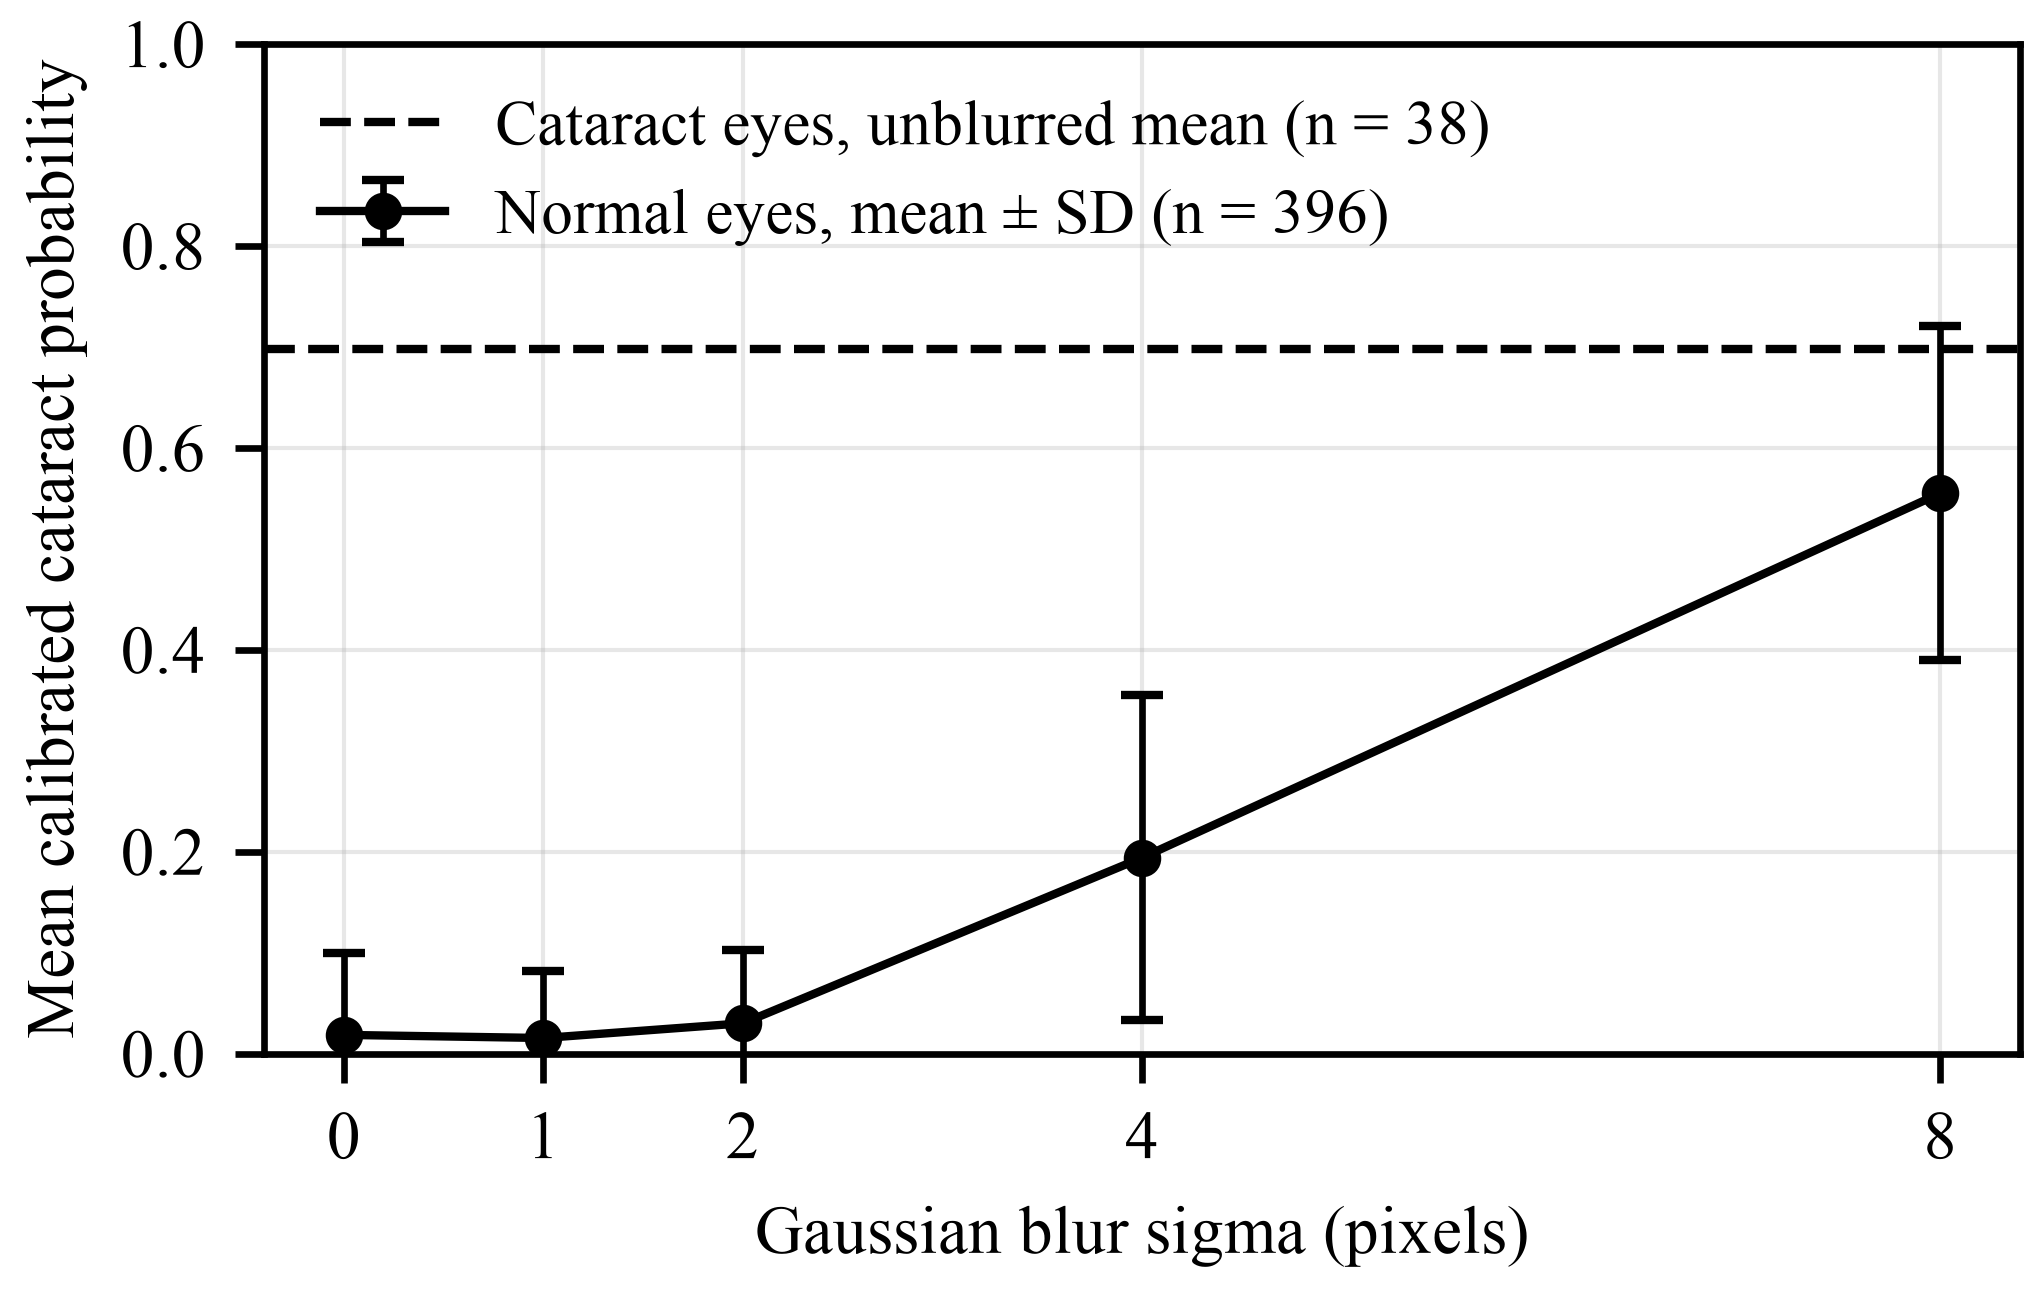
\includegraphics[width=\linewidth]{figures/blur.png}
\caption{Synthetic blur test. Mean calibrated cataract probability of the 396 normal-fundus validation eyes, with standard deviation, at increasing Gaussian blur, compared with the unblurred mean of the 38 validation cataract eyes (dashed line).}\label{fig:1}
\end{figure}

We then drew Grad-CAM heatmaps \cite{ref10} for the cataract output of the application model, using
its last convolutional block, on 21 photographs selected by a rule fixed in advance: the first three
photographs by file name in each of seven groups. The groups were normal internal test eyes with
each of the three decisions, referred cataract eyes, and media-opacity eyes with each of the three
decisions. There is no group of missed cataract eyes because all 31 eligible cataract eyes in the
internal test split were referred. As in the blur test, eligible eyes had cataract as their only
diagnosis and no media-opacity, image-quality or exclusion flag, which leaves 31 of the 40 test
cataract eyes. In most heatmaps, including those of normal eyes, the strongest activation lay along
the upper edge of the circular fundus image (Fig.~\ref{fig:2}, a to d), and some referred
photographs also showed broad activation over hazy regions. Each heatmap is scaled to its own range,
so its colours show where the model looked within one photograph, not how strong the evidence was.
The heatmaps suggest that the cataract head may respond to features of the image edge or to overall
image quality as well as to cataract. This is consistent with the media-opacity and blur results,
but the heatmaps are supporting observations only.

Both predefined warnings were triggered. The final assessment of the three checks concluded that
there is a potential haze-related shortcut or image-quality robustness concern, but that the causal
mechanism remains inconclusive, and it recommended further controlled tests and team review before
any conclusion is drawn about clinical use.

\begin{figure}[t]
\centering
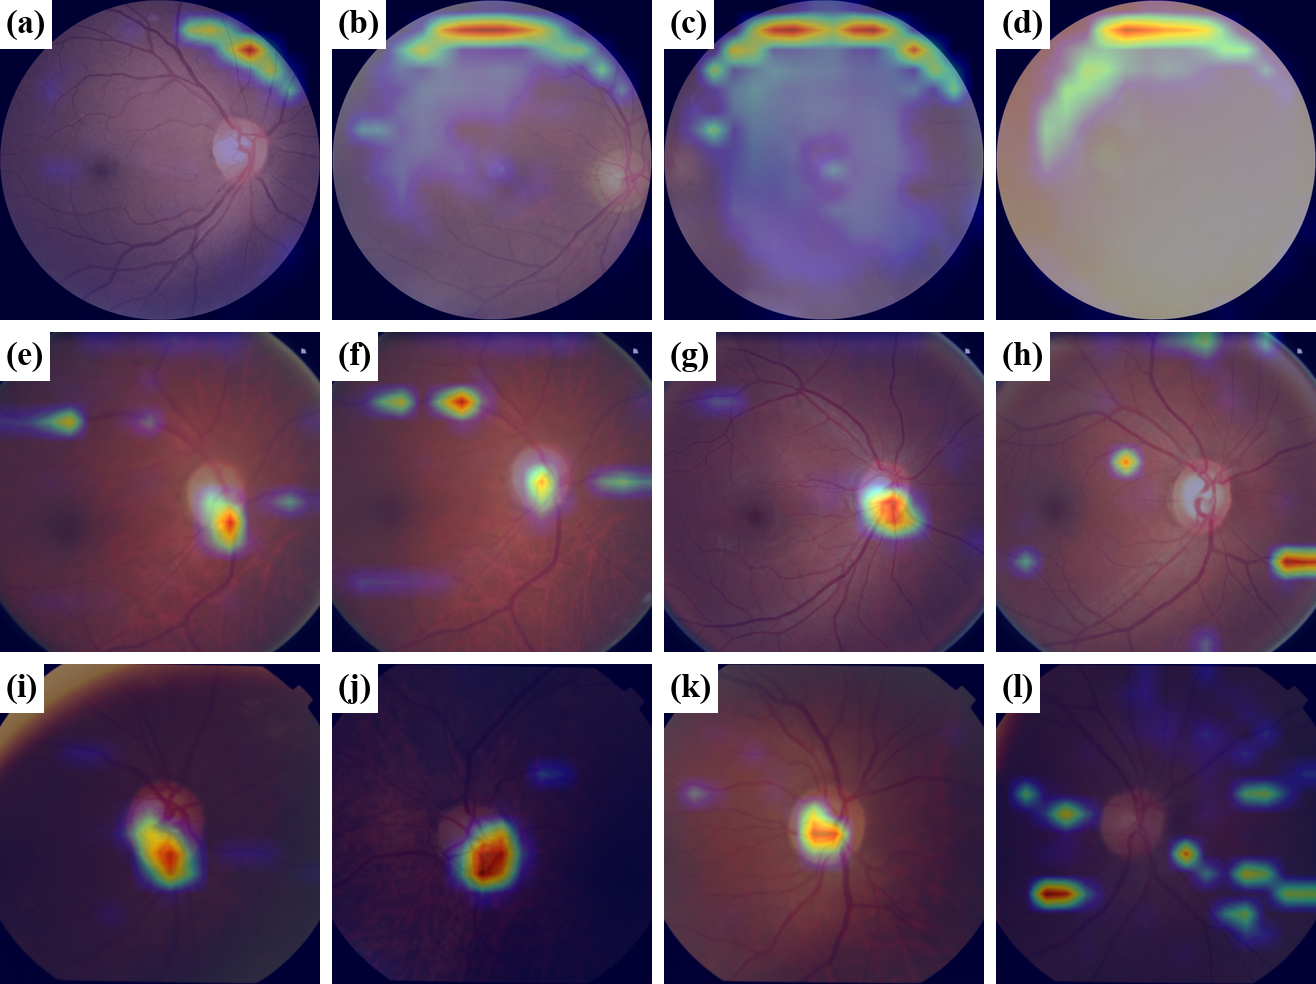
\includegraphics[width=\linewidth]{figures/heatmaps.png}
\caption{Grad-CAM heatmaps of the application model. Top, cataract output on internal test eyes (first eye of four predefined groups): (a) normal, No concern; (b) normal, Refer; (c) cataract, Refer; (d) media opacity, Refer. Middle, glaucoma output on ORIGA; bottom, on DRISHTI-GS: (e, i) glaucoma, peak inside the disc outline (not drawn); (f, j) glaucoma, peak outside; (g, k) healthy, inside; (h, l) healthy, outside. The glaucoma examples were chosen to show each outcome and are not a representative sample.}\label{fig:2}
\end{figure}

For glaucoma, an optic disc check asked whether the glaucoma output of the application model attends
to the optic disc, where glaucomatous damage is visible on a fundus photograph. Grad-CAM heatmaps of
the glaucoma output, taken from the same last convolutional block, were drawn for all 650 ORIGA and
101 DRISHTI-GS photographs, the two external sets that include optic disc outlines. A hit was
counted when the strongest point of the heatmap fell inside the disc outline, after the outline had
been cropped and resized in the same way as the photograph. The peak fell inside the disc in 240 of
650 ORIGA photographs (36.9\%) and 68 of 101 DRISHTI-GS photographs (67.3\%); Fig.~\ref{fig:2} (e to
l) shows examples of both outcomes. This is far more often than a uniformly random peak location
would produce, since the disc covers only about 2.4\% and 3.7\% of the 512 \(\times\) 512 image,
respectively. Hits were more common in glaucoma eyes than in healthy eyes: 94 of 168 (56.0\%)
against 146 of 482 (30.3\%) on ORIGA, and 50 of 70 (71.4\%) against 18 of 31 (58.1\%) on DRISHTI-GS.
The DRISHTI-GS outline is a soft map, in which pixels with a value of 128 or more were counted as
disc; cut-offs of 1 and 255 gave hit rates of 69.3\% and 64.4\%. The glaucoma head therefore often
attends to the optic disc, more so in glaucoma eyes, but on ORIGA the peak lay outside the disc in
most photographs. As with the cataract heatmaps, these results describe where the model looks, not
what drives its decisions.

\section{Application}

\pendingedit{DUAL includes a prototype web application for clinic staff. [Pending: final description once the
application features are complete.]} A user selects a patient and the left or right eye, and uploads
one fundus photograph as a JPG or PNG file of up to 20 MB. The application runs the quality check,
stores the original photograph and its 512 \(\times\) 512 preprocessed copy, and scores the
photograph. For each condition, it shows the result (No concern, Refer, or Uncertain, refer), the
calibrated risk score with its threshold, and a Grad-CAM heatmap \cite{ref10} of the regions that
most influenced the score. Past screenings are listed on a History page.

Fig.~\ref{fig:3} shows how the application connects to the data, model and evaluation pipeline. The
front end is a React application built with Vite and hosted on Vercel. It calls a back end written
in Python with FastAPI and hosted on Render, which provides 20 REST endpoints for sign-in, patients,
photographs, screenings, PDF exports and model information. Records are stored in a PostgreSQL
database on Supabase, and photographs and heatmaps are kept in private Supabase Storage buckets that
the browser can reach only through the API. Staff passwords are stored as PBKDF2 hashes, and
sessions use an HttpOnly cookie that expires after 12 hours. \pendingedit{Sign-in and PDF export of screening and
patient summaries are implemented and tested in the back end, but the front end does not yet include
a sign-in page or an export button. [Pending: update once the sign-in page and PDF export are added
to the front end.]}

\pendingedit{In the current version, the back end uses a stand-in model that returns placeholder scores and
heatmaps, clearly marked as mock, so that the whole workflow can be tested end to end. Connecting
the frozen shared model (seed 42) and its calibration to the application is planned for the final
sprint. [Pending: update once the frozen model and its calibration are connected to the
application.]} The application contains only fictitious patient records and is intended for academic,
non-commercial use.

\begin{figure*}[t]
\centering
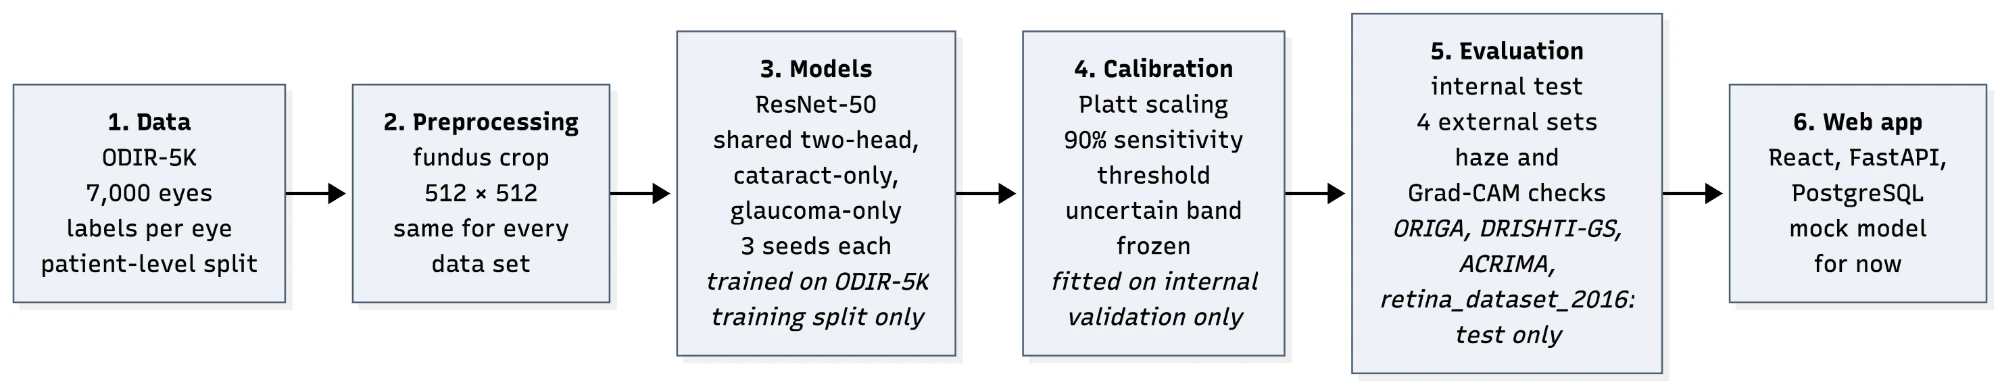
\includegraphics[width=\linewidth]{figures/pipeline.png}
\caption{Overview of the DUAL pipeline, from data to the screening application.}\label{fig:3}
\end{figure*}

\section{Limitations}

External cataract testing relies on a single data set, retina\_dataset\_2016, which has 100 cataract
photographs and on which the application model reached an AUROC of 0.909. Glaucoma, by contrast, was
tested on three external data sets in addition to retina\_dataset\_2016. Conclusions about how well
cataract detection generalises are therefore weaker than those for glaucoma.

The retina\_dataset\_2016 collection has no documented origin or licence, and ACRIMA contains tight
optic disc crops rather than full fundus photographs like those used in training. The folder labels
of retina\_dataset\_2016 have not been clinically verified and should not be treated as adjudicated
ground truth. The copy we used is kept in the team repository with a SHA-256 hash for every image.
Both data sets are reported in separate rows, and ACRIMA was left out of the optic disc heatmap
check. Because every model scored near or below chance on ACRIMA, it says little about how the
models handle full fundus photographs.

All training data come from a single source, ODIR-5K. Its labels were derived from free-text
diagnostic keywords for each eye and were not regraded by specialists, so some labels may be wrong.
Suspected-glaucoma eyes were excluded from both classes, and the media-opacity eyes were held out
for the haze check, so the model has not learned how to handle these borderline cases.

The validation split was used to choose the best epoch, to fit the calibration and to set the
thresholds and the uncertainty margin, so validation figures are optimistic. Calibration was fitted
on ODIR-5K only and did not hold on the external sets, where the calibrated probabilities were far
below the proportion of positive photographs. The risk score shown in the application should
therefore not be read as a probability for photographs from other sources. Small differences between
CPU and GPU scores were observed when validation scores were reproduced. Because each threshold sits
at a validation probability, such differences can move individual eyes across a threshold.

At the frozen settings, the application model would refer about 42\% of internal test eyes, mostly
for glaucoma, where specificity was 67\%. The 90\% sensitivity floor was set on only 39 validation
glaucoma eyes, and one of the three shared seeds fell below it on the test split. We accepted this
referral load to keep missed cases low, but it would place a heavy burden on a real screening
service.

On the external sets, the application model no longer met the 90\% sensitivity floor: it referred
73.0\% of external cataract-positive photographs and 69.6\% to 77.1\% of glaucoma-positive
photographs on the full fundus sets. The thresholds were not refitted, because tuning on external
data would bias the test, but a screening service would need thresholds checked on its own cameras
and patients. The external label files also lack patient identifiers, so the external intervals
treat both eyes of a person as independent and may be too narrow.

The cataract head referred 86\% of the media-opacity eyes, which are graded as not cataract, and
93\% of normal eyes once they were blurred with a Gaussian filter of sigma 4. Its Grad-CAM heatmaps
were often strongest at the upper edge of the image. The glaucoma heatmaps peaked inside the optic
disc in only 37\% of ORIGA photographs, so the glaucoma head may also rely on evidence away from the
disc. Hazy or blurred photographs without cataract are therefore likely to be referred, and on data
sets where cataract photographs are also hazier, cataract results may overstate the model's true
ability to recognise cataract.

DUAL screens for only two conditions, from one photograph per eye, and does not grade severity. It
is a triage aid for deciding who should see a specialist, not a diagnostic device, and it has not
been validated in a clinical setting.

\section{Conclusion and Future Work}

DUAL screens one fundus photograph for cataract and glaucoma with a single shared network and gives
a triage decision for each condition. With calibration, thresholds and an abstention band fixed on
internal validation before testing, the application model reached internal test AUROCs of 0.995 for
cataract and 0.921 for glaucoma and referred all 40 cataract eyes and 43 of 45 glaucoma eyes. The
shared backbone performed as well as separate single-disease models, with no consistent winner on
external data. The external results were weaker. On four public data sets, the AUROC fell to 0.909
for cataract and to between 0.760 and 0.869 for glaucoma on full fundus photographs, sensitivity
dropped below the 90\% floor, and the calibrated probabilities did not transfer. The shortcut checks
raise further concerns: the cataract head refers most hazy or blurred photographs without cataract,
and the glaucoma heatmaps peak on the optic disc in only some of the photographs. DUAL is a research
prototype and is not ready for clinical screening.

Several directions for future work follow from these results. External cataract testing needs a
second labelled data set, such as AREDS2, which requires institutional access. Thresholds and
calibration should be checked on photographs from each new camera and population before use, ideally
with patient identifiers so that confidence intervals account for both eyes of a person. Training
with media-opacity and blurred photographs labelled as not cataract, or with image-quality labels,
could reduce the sensitivity to haze, and disc-centred images, as used by G-RISK \cite{ref9}, could
make glaucoma detection more stable across data sets. \pendingedit{Finally, connecting the frozen model to the
web application and testing it with clinic staff would show whether the referral load is workable in
practice. [Pending: revise once the model connection and application testing are complete.]}

\section*{AI Use Disclosure}

Generative AI assistants were used as support tools during this project, as allowed by the course
instructor when their use is disclosed. \pendingedit{They helped with drafting and editing project documents,
writing and reviewing parts of the code and tests, checking references and preparing tables and
figures. [Pending: confirm once every team member has reported their AI use.]} Every AI-assisted
output was checked and edited by a team member before it was used or submitted. The team made all
project decisions and is responsible for the code, the documentation and the results it presents.
Every reported result comes from the team's committed code and result files.

\begin{thebibliography}{99}

\bibitem{ref1}

GBD 2019 Blindness and Vision Impairment Collaborators and Vision Loss Expert Group of the Global
Burden of Disease Study, "Causes of blindness and vision impairment in 2020 and trends over 30
years, and prevalence of avoidable blindness in relation to VISION 2020: the Right to Sight: an
analysis for the Global Burden of Disease Study," Lancet Glob. Health, vol. 9, no. 2, pp. e144-e160,
2021.

\bibitem{ref2}

Y.-C. Tham et al., "Detecting visually significant cataract using retinal photograph-based deep
learning," Nat. Aging, vol. 2, no. 3, pp. 264-271, 2022.

\bibitem{ref3}

Y.-C. Tham, X. Li, T. Y. Wong, H. A. Quigley, T. Aung, and C.-Y. Cheng, "Global prevalence of
glaucoma and projections of glaucoma burden through 2040: a systematic review and meta-analysis,"
Ophthalmology, vol. 121, no. 11, pp. 2081-2090, 2014.

\bibitem{ref4}

Z. Soh et al., "The global extent of undetected glaucoma in adults: a systematic review and
meta-analysis," Ophthalmology, vol. 128, no. 10, pp. 1393-1404, 2021.

\bibitem{ref5}

D. S. W. Ting et al., "Development and validation of a deep learning system for diabetic retinopathy
and related eye diseases using retinal images from multiethnic populations with diabetes," JAMA,
vol. 318, no. 22, pp. 2211-2223, 2017.

\bibitem{ref6}

Z. Li, Y. He, S. Keel, W. Meng, R. T. Chang, and M. He, "Efficacy of a deep learning system for
detecting glaucomatous optic neuropathy based on color fundus photographs," Ophthalmology, vol. 125,
no. 8, pp. 1199-1206, 2018.

\bibitem{ref7}

H. Liu et al., "Development and validation of a deep learning system to detect glaucomatous optic
neuropathy using fundus photographs," JAMA Ophthalmol., vol. 137, no. 12, pp. 1353-1360, 2019.

\bibitem{ref8}

J. H. L. Goh et al., "Artificial intelligence for cataract detection and management," Asia-Pac. J.
Ophthalmol., vol. 9, no. 2, pp. 88-95, 2020.

\bibitem{ref9}

R. Hemelings et al., "A generalizable deep learning regression model for automated glaucoma
screening from fundus images," npj Digit. Med., vol. 6, Art. no. 112, 2023.

\bibitem{ref10}

R. R. Selvaraju, M. Cogswell, A. Das, R. Vedantam, D. Parikh, and D. Batra, "Grad-CAM: visual
explanations from deep networks via gradient-based localization," in Proc. IEEE Int. Conf. Comput.
Vis. (ICCV), 2017, pp. 618-626.

\bibitem{ref11}

M. Christopher et al., "Performance of deep learning architectures and transfer learning for
detecting glaucomatous optic neuropathy in fundus photographs," Sci. Rep., vol. 8, Art. no. 16685,
2018.

\bibitem{ref12}

A. Diaz-Pinto, S. Morales, V. Naranjo, T. Köhler, J. M. Mossi, and A. Navea, "CNNs for automatic
glaucoma assessment using fundus images: an extensive validation," Biomed. Eng. Online, vol. 18,
Art. no. 29, 2019.

\bibitem{ref13}

L. Zhang et al., "Automatic cataract detection and grading using deep convolutional neural network,"
in Proc. IEEE 14th Int. Conf. Netw., Sens. Control (ICNSC), 2017, pp. 60-65.

\bibitem{ref14}

R. Caruana, "Multitask learning," Mach. Learn., vol. 28, no. 1, pp. 41-75, 1997.

\bibitem{ref15}

L.-P. Cen et al., "Automatic detection of 39 fundus diseases and conditions in retinal photographs
using deep neural networks," Nat. Commun., vol. 12, Art. no. 4828, 2021.

\bibitem{ref16}

N. Li, T. Li, C. Hu, K. Wang, and H. Kang, "A benchmark of ocular disease intelligent recognition:
one shot for multi-disease detection," in Benchmarking, Measuring, and Optimizing (Bench 2020),
Lecture Notes in Computer Science, vol. 12614. Cham, Switzerland: Springer, 2021, pp. 177-193.

\bibitem{ref17}

J. R. Zech, M. A. Badgeley, M. Liu, A. B. Costa, J. J. Titano, and E. K. Oermann, "Variable
generalization performance of a deep learning model to detect pneumonia in chest radiographs: a
cross-sectional study," PLoS Med., vol. 15, no. 11, Art. no. e1002683, 2018.

\bibitem{ref18}

R. Geirhos et al., "Shortcut learning in deep neural networks," Nat. Mach. Intell., vol. 2, no. 11,
pp. 665-673, 2020.

\bibitem{ref19}

A. J. DeGrave, J. D. Janizek, and S.-I. Lee, "AI for radiographic COVID-19 detection selects
shortcuts over signal," Nat. Mach. Intell., vol. 3, no. 7, pp. 610-619, 2021.

\bibitem{ref20}

C. Guo, G. Pleiss, Y. Sun, and K. Q. Weinberger, "On calibration of modern neural networks," in
Proc. 34th Int. Conf. Mach. Learn. (ICML), PMLR vol. 70, 2017, pp. 1321-1330.

\bibitem{ref21}

C. Leibig, V. Allken, M. S. Ayhan, P. Berens, and S. Wahl, "Leveraging uncertainty information from
deep neural networks for disease detection," Sci. Rep., vol. 7, Art. no. 17816, 2017.

\bibitem{ref22}

Z. Zhang et al., "ORIGA-light: an online retinal fundus image database for glaucoma analysis and
research," in Proc. Annu. Int. Conf. IEEE Eng. Med. Biol. Soc. (EMBC), 2010, pp. 3065-3068.

\bibitem{ref23}

J. Sivaswamy, S. R. Krishnadas, G. D. Joshi, M. Jain, and A. U. S. Tabish, "Drishti-GS: retinal
image dataset for optic nerve head (ONH) segmentation," in Proc. IEEE 11th Int. Symp. Biomed.
Imaging (ISBI), 2014, pp. 53-56.

\bibitem{ref24}

retina\_dataset (fundus images labelled normal, cataract, glaucoma and retina disease; no documented
clinical source, grading method or licence), GitHub repository, 2016. Original repository
sjchoi86/retina\_dataset removed; surviving copy with the original November 2016 commit history
used: \url{https://github.com/yiweichen04/retina_dataset} (accessed Sep. 2026).

\bibitem{ref25}

K. He, X. Zhang, S. Ren, and J. Sun, "Deep residual learning for image recognition," in Proc. IEEE
Conf. Comput. Vis. Pattern Recognit. (CVPR), 2016, pp. 770-778.

\bibitem{ref26}

J. Deng, W. Dong, R. Socher, L.-J. Li, K. Li, and L. Fei-Fei, "ImageNet: a large-scale hierarchical
image database," in Proc. IEEE Conf. Comput. Vis. Pattern Recognit. (CVPR), 2009, pp. 248-255.

\bibitem{ref27}

D. P. Kingma and J. Ba, "Adam: a method for stochastic optimization," in Proc. 3rd Int. Conf. Learn.
Represent. (ICLR), 2015, arXiv:1412.6980.

\bibitem{ref28}

J. C. Platt, "Probabilities for SV machines," in Advances in Large-Margin Classifiers, A. J. Smola,
P. Bartlett, B. Schölkopf, and D. Schuurmans, Eds. Cambridge, MA, USA: MIT Press, 2000, pp. 61-74.

\end{thebibliography}

% Team revision log. Comment out the next line for a manuscript-only build.

% !TeX root = paper.tex
\clearpage\onecolumn\section*{Version History}
\begingroup
\small
\renewcommand{\arraystretch}{1.2}
\begin{longtable}{|l|p{0.14\linewidth}|p{\dimexpr0.86\linewidth-4em-6\tabcolsep-4\arrayrulewidth\relax}|}
\hline
\textbf{Version} & \textbf{Date} & \textbf{Changes} \\ \hline
\endhead
0.1 & 7 October 2026 & Starting file: IEEE layout and section headings. \\ \hline
0.2 & 8 October 2026 & Sections III (Data) and IV (Labels and Splits) drafted. \\ \hline
0.3 & 9 October 2026 & Section V (Preprocessing) drafted \\ \hline
0.4 & 23 October 2026 & Sections VI (Model and Training), VII (Calibration, Thresholds and Abstention), IX (Application) and X (Limitations) drafted from the repository. Missing full stop added in Section V. \\ \hline
0.5 & 28 October 2026 & Sections VIII-A (Internal Test, with Table~\ref{tab:I}), VIII-C (Multi-Task vs Single-Task Ablation) and VIII-D (Calibration and Abstention) drafted from the Task 13 results. External protocol paragraph added to VIII-B. VIII-E renamed and media-opacity haze check added from PR 85. Two limitations added. \\ \hline
0.6 & 29 October 2026 & Sections I (Introduction) and II (Literature Review) drafted. Citations numbered in order of first use and the reference list added (28 entries, each checked against PubMed, Crossref or the publisher). \\ \hline
0.7 & 30 October 2026 & VIII-E: synthetic blur result added from PR 86 (open); media-opacity figures confirmed against merged PR 85. Haze limitation and one sentence in Section II updated to match. \\ \hline
0.8 & 31 October 2026 & VIII-B: external results and Table~\ref{tab:II} added from PR 87 (open). VIII-E: Grad-CAM heatmap paragraph added from PR 88 (open); blur figures confirmed against merged PR 86. Abstract drafted. Limitations updated for the external results, and one new limitation added. \\ \hline
0.9 & 3 November 2026 & VIII-E: final haze verdict added from SCRUM-100 (PR 89); heatmap paragraph confirmed against merged PR 88. All Task 15 results are now on main (PR 91). Two-column layout restored for the body (lost in v0.6). \\ \hline
0.10 & 6 November 2026 & VIII-E: optic disc heatmap check added from Task 16 (PR 92, merged to develop). VIII-B: external figures confirmed against merged PR 87. Section XI (Conclusion and Future Work) drafted. Abstract and one limitation updated. Section IX checked against the merged back end (PR 90). All 28 references rechecked against Crossref, PubMed, arXiv, PMLR and GitHub; titles corrected for \cite{ref28} (published chapter title) and wording for \cite{ref24}. Every cited claim checked against its source; wording tightened for \cite{ref6}, \cite{ref17} and \cite{ref18}, and the LNCS volume added to \cite{ref16}. Final clean-up: all open notes resolved or removed, Fig.~\ref{fig:1} (pipeline diagram) added, training details and the AI use disclosure written, and contribution (6) corrected to match Section IX. Review fixes: application described as a prototype with a mock model, freeze and run records cited by commit, protocol draft status and the earlier 21-eye trial disclosed, dataset exclusion list shortened, fellow-eye design explained, retina\_dataset\_2016 limits stated, optic disc baseline qualified, AI disclosure revised, and some wording simplified. \\ \hline
0.11 & 10 November 2026 & Task 17: abstract, VIII-C and conclusion updated to match the shared versus single-task comparison in PR 95 (open, 9 November); all its figures already matched Tables I and II. 9 November: every reported figure rechecked against the repository (main at 1222b7d); one sentence in VIII-B corrected, since the external differences between designs were not mostly within the spread between seeds; wording edited throughout for clarity and consistency. Layout aligned with the IEEE template: two empty paragraphs removed from Section IV, Section V spacing matched to the rest, table text, captions and references set to 8 pt, abstract text no longer italic. 10 November: points from the team review addressed. IV now says where the other two cataract eyes are. VII explains the uncertain label and the choice of seed 42. VIII-B corrects the ACRIMA wording, and VIII-E states the eligibility rules and both warning criteria. Section IX separates back-end and front-end features. Table~\ref{tab:II} columns widened (rebalanced again for 9 pt text). The abstract wording on cataract was revised, and pending notes in square brackets were added to the yellow parts. Contribution (5) now lists all shortcut checks. VIII-C now reports the paired AUROC differences from the Task 17 analysis (PR 95, head 7178102, approved 10 November). Formatting matched to the course IEEE template: paragraphs indented with no extra space between them, table text 9 pt, table captions on two lines in title case, journal and proceedings names in italic, author emails added in 9 pt Courier, title block spacing matched, and Times New Roman set as the font for the whole document. All spacing then checked element by element against the template styles: heading, caption, figure, abstract and reference spacing matched, level-2 headings and references use hanging indents, and table header cells are centred after the first column. Tables I and II are set to stay on one page with their captions. Two figures added to VIII-E from the merged Task 15 and Task 16 results: Fig.~\ref{fig:1}, the synthetic blur test, redrawn at column size from results/task15/synthetic\_blur\_summary.csv, and Fig.~\ref{fig:2}, a Grad-CAM panel built from results/task15/cataract\_heatmaps and results/task16/glaucoma\_heatmap\_contact\_sheet.png. The pipeline figure is now Fig.~\ref{fig:3}. Page size changed from US Letter to A4 to match the course template, with its margins (0.75 in top, 0.56 in sides, 1.69 in bottom) and column gap; Table~\ref{tab:II} and this table narrowed slightly to fit. Table~\ref{tab:II} moved below the last paragraph of VIII-B and Fig.~\ref{fig:2} moved above the optic disc paragraph, so that neither is split or leaves a gap in a column. \\ \hline
\end{longtable}
\endgroup


\end{document}
